\subsection{Activating the fan}\label{subsec:activating-the-fan}

In order to effectively distribute and more efficiently evaporate the formic acid, a fan is used.
This requirement is fulfilled, when a fan can be controlled by the processor.
Furthermore, it must spin directly after the formic acid has been distributed by the pump.
It must do so for a minute, to ensure a good distribution.

The fan itself is powered by the previously mentioned powerbank, since the processor cannot power multiple high loads.
A relay implements a switch that can be controlled by the microprocessor.
The microprocessor's and the fan's circuits are disconnected by this relay.
If a pump cycle starts, the processor closes the fans circuit via the relay for one minute, before opening it again.

\begin{lstlisting}[label={lst:fan-control},language=C++, caption=Controling the fan]
void loop() {
    ...
    if (millis() - lastPumpCycle >= ONE_HOUR) {
        ...
        lastPumpCycle = millis();
        fanStartTime = millis();
    }
    if (millis() - fanStartTime < ONE_MINUTE) {
        ...
        getRealIO()->on(FAN);
    } else {
        ...
        getRealIO()->off(FAN);
    }
    ...
}
\end{lstlisting}

Listing \ref{lst:fan-control} shows the algorithm that controls this behaviour.
If between the current time and the last pump cycle is more than an hour, the times are set the current time.
Doing so allows the program to know when the last cycle ended and measure if the next should begin.
Immediately afterwards, it is checked whether between the current time and the fan start time is a minute.
If that is not the case, the pin referenced by the constant \textit{FAN} is set to output a signal, triggering the relay.
This constant is a number, which references the pin as described by the physical layout of the processor.
If between the current time and the fan start time is a minute, the fan is turned off again.

\begin{figure}
    \centering
    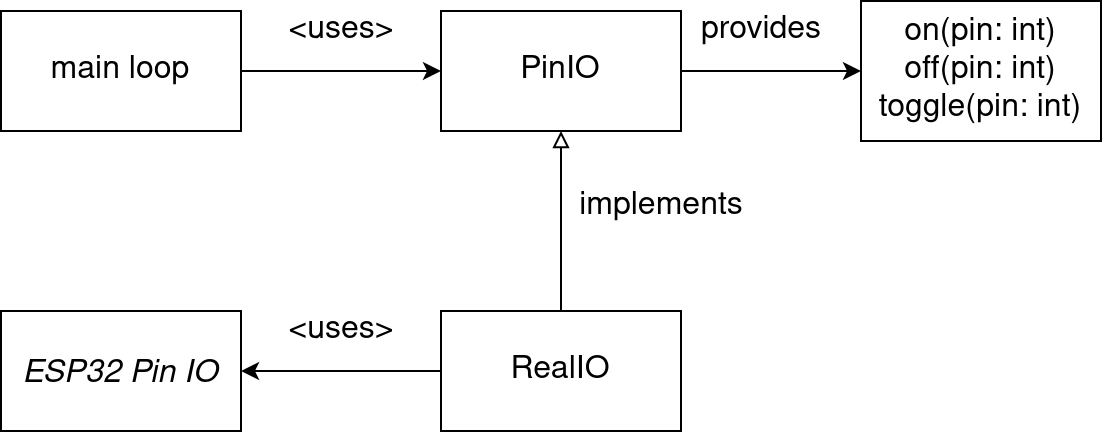
\includegraphics[width=0.5\textwidth]{img/realio-interaction}
    \caption{Abstraction of the pin IO and its usage}
    \label{fig:abstraction-of-pinio}
\end{figure}

Similar to section \ref{subsec:reading-temperature}, the interaction between the main loop and the actual pin IO of the ESP32 is too convoluted to show in code.
Therefore, Figure \ref{fig:abstraction-of-pinio} shows a visual representation.
The actual interaction with the pin IO is implemented by a \textit{RealIO} class.
This class implements a \textit{PinIO} interface, which provides the methods \textit{on}, \textit{off}, and \textit{toggle}.
These can then be used the main loop to interact with the physical pins.
